\section{Limitations of Current Practice in Multi-Streamed SSDs}
In this section, we review the key weaknesses of existing stream management techniques 
as well as stream implementation methods.  
PCStream was motivated to overcome these weaknesses so that multi-streamed
SSDs can be widely employed in practice.

\subsection{No Automatic Stream Management for General I/O Workloads}
Most existing stream management techniques~\cite{MultiStream, Level, vStream} 
require programmers to manually allocate streams for their applications.

{\color{blue}
For example, 
in both ManualStream and vStream, there is no systematic guildeline on how to
allocate streams for a given application. 
The efficiency of stream allocations largely depends on the programmer's 
understanding and expertise on data temperature (i.e., frequency of updates)
and internals of file systems/database systems.
}
Furthermore, these
techniques also assume that the number of streams is known {\it a priori}.  
Therefore, when an SSD with a different number of streams is used, 
these techniques need to re-allocate streams manually.
A recently proposed \textsf{\small vStream}~\cite{vStream} 
technique is an exception to this 
restriction by allocating streams to virtual streams, not physical streams.  
However, even in \textsf{\small vStream}, virtual stream allocation is left to
programmer's decisions.

{\color{blue}
Although \textsf{\small FStream} and \textsf{\small AutoStream} may be considered 
as automatic stream management techniques,
their applicability is quite limited.
\textsf{\small FStream} can be useful for separating file system metadata but it does not
work for the user data separation.
\textsf{\small AutoStream}~\cite{AutoStream} is the only known technique that works in a 
fully automatic fashion by making stream allocation decisions within 
the kernel.
However, since \textsf{\small AutoStream} predicts data lifetimes using the
access frequency of the same LBA, \textsf{\small AutoStream} does not work
well with recent data-intensive 
applications where a majority of
new data are written in an append-only manner.  
}

In order to illustrate a mismatch between an LBA-based predictor and 
append-only workloads, we analyzed the write pattern of 
RocksDB~\cite{RocksDB}, which is a
popular key-value store based on the LSM-tree algorithm~\cite{LSM}.
Fig.~\ref{fig:lba_lifetime}(a) shows how LBAs may be related 
to data lifetimes in RocksDB~\cite{RocksDB}.  
{\color{blue}
We define the lifetime of data as the interval length (in terms of
the logical time based on the number of writes) between
the data is first written and when the data is invalidated
by an overwrite or a TRIM command.
}
As shown in Fig.~\ref{fig:lba_lifetime}(a), 
there is no strong correlation between LBAs and lifetimes in RocksDB.  
This scatter plot is in sharp contrast with one for update workloads 
where a few distinct LBA regions have short lifetimes while others 
have very long lifetimes.

\begin{figure}[t]
	\centering
	\hfill
	%\vspace{-9pt}
	%\captionsetup[subfigure]{margin={0cm,1cm}}
	\subfloat[Lifetime patterns over LBAs]{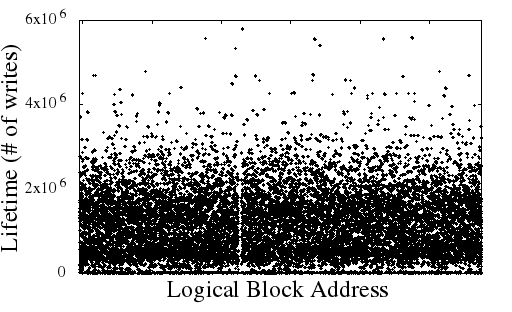
\includegraphics[width=0.215\textwidth]{figure/lba_lifetime2}}  % data from 0/03031641
	\hspace{10pt}
	\subfloat[Lifetime patterns over time]{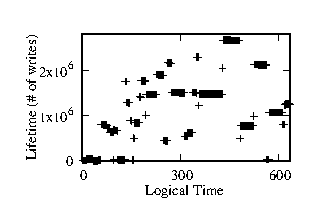
\includegraphics[width=0.21\textwidth]{figure/lifetime_in_chunk}}
	%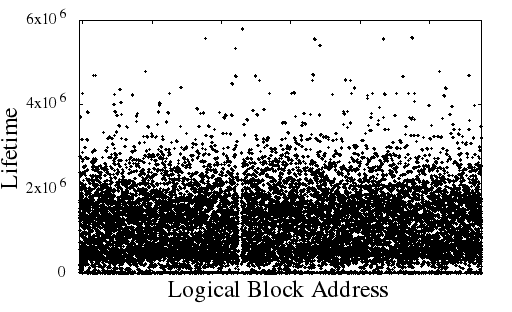
\includegraphics[width=0.9\linewidth]{figure/lba_lifetime} 
	%\vspace{-3pt}
	\caption{Lifetime distributions of append-only workload over addresses and times.} %shane part
	\label{fig:lba_lifetime}
	%\vspace{-20pt}
\end{figure}


We also analyzed 
if the lifetimes of LBAs change under some predictable patterns over time 
although the overall lifetime distribution shows large variances.
Fig.~\ref{fig:lba_lifetime}(b) shows a scatter plot of data lifetimes over the logical time 
for a specific 1-MB chunk with 256 pages. 
As shown in Fig.~\ref{fig:lba_lifetime}(b), 
for the given chunk, data lifetimes vary in a random fashion
(although some temporal locality is observed).
Over the logical time, the lifetime of data written to the chunk 
varies in an unpredictable fashion.  
For example, at the logical time 10, the lifetime was 1 but it increases about 
2.6 million around the logical time 450 
followed by a rapid drop around the logical time 600. 
Our illustration using RocksDB strongly suggests that under append-only workloads, 
{\color{blue}LBAs are not meaningful in predicting data lifetimes reliably.
In order to support {\it general} I/O workloads in an automatic fashion, stream 
management decisions should be based on higher-level information
which do not depend on lower-level details such as write patterns of successive LBAs.
}

\subsection{Limited Number of Supported Streams}
One of the key performance parameters in multi-streamed SSDs is the number of 
available streams in SSDs.  
Since the main function of  streams is to separate data with different lifetimes 
so that they are not mixed in the same block, it is clear that the 
higher the number of streams, the more efficient the performance of multi-streamed SSDs.
For example, the SSD performance keeps improving as the number of streams increases 
until data with different lifetimes are allocated to separate streams.   
In order to support a large number of streams, the SBC-4 and NVMe revision 1.3, which define the 
multi-stream related specifications, allow up to 65,536 streams~\cite{T10, NVMe}.  
However, the number of streams supported in
commercial SSDs is quite limited, say, 4 to 16~\cite{MultiStream, Level, AutoStream}, 
{\color{blue}
because of several implementation constraints such as backup power capacity and the memory size.
In the SSD, a write buffering mechanism is commonly used to manage the size difference 
between the FTL mapping unit and the flash program unit and to efficiently utilize 
the high-degree of SSD internal parallelism for high performance. 
And the buffering mechanism requires a backup power resource and a fast memory resource.

In data centers or storage servers where multi-streamed SSDs are used,
in order to guarantee the data integrity even under sudden power-off conditions, 
SSDs use tantalum or electrolytic capacitors as a backup power source.  
When a main power is suddenly failed, the backup power is used to write back the
buffered data reliably.  
Since the capacity of backup power is limited because of the limited PCB size and 
its cost, the maximum amount of buffered data is also limited.  
In multi-streamed SSDs where
each stream needs its own buffered area, the amount of buffered data increases 
as the number of streams increases.  
The practical limit in the capacity of backup power, therefore, dictates the maximum
number of streams as well.

The limited size of fast memory, such as TCM or SRAM, is another main hurdle in increasing 
the number of streams in multi-streamed SSDs.
Since multi-stream related metadata which includes data structes for write buffering 
should be accessed quickly as well as frequently, 
most SSD controllers implement multi-stream data structures on fast memory than more common DRAM. 
Since the buffered write data is the latest data, 
it is always necessary to check whether there is requested LBA 
among the buffered data at the time of read request processing.
To effectively implement this check process, a hash table or bloom filter can be used, 
and buffered LBA information and buffer address are managed.
Placing these data structures in slower memory is not desirable 
because the read processing speed is greatly reduced.  
Furthermore, these data structures are also referred to store buffered data in NAND flash, 
the data structures must be located in fast memory for high write throughput. 
However, most SSD manufacturers are quite sensitive in increasing the size of 
fast memory because it may increase the overall SSD cost.   
A limited size of fast memory, unfortunately, restricts the number of
supported streams quite severely.
}

